%SourceDoc ws-skript.tex
%
% c03-erwartung.tex
%
% (c) 2006 Prof. Dr. Andreas Mueller
% $Id: c03-erwartung.tex,v 1.18 2008/11/02 00:12:44 afm Exp $
%
\rhead{Erwartung und Varianz}
\chapter{Erwartungswert und
Varianz\label{chapter-erwartungswert-und-varianz}} F"ur den
\marginpar{\tiny\raggedright Erwarteter Gewinn im Casino}
\index{Casino}
Casinobetreiber ist die genaue Wahrscheinlichkeit eines Ereignisses
nur von sekund"arem Interesse. Sein Betrieb ist genau dann rentabel,
wenn im Mittel, "uber viele Spiele, die Spieler mehr Geld in seinem
Etablissement liegen lassen als er an Gewinnen auszahlen muss.
Zun"achst wird er sich dazu Gedanken machen, welchen Gewinn jede
einzelne Spielsituation f"ur ihn ergibt. Zusammen mit der
Wahrscheinlichkeit des Eintretens dieser Situation wird er abzusch"atzen
versuchen, wie gross sein Gewinn im Mittel sein wird.

Ganz "ahnlich geht es dem Experimentator, der eine Messung mehrmals
durch\-f"uhrt.  Er kann nicht davon ausgehen, dass jede Messung das
gleiche Resultat liefert.  Jede einzelne Messung ist
ein Wahrscheinlichkeitsexperiment mit einer sehr
grossen Zahl von Einfl"ussen, die alle nicht bekannt sind. Der
Experimentator wird versuchen, aus einer grossen Zahl von Messresultaten
einen besonders wahrscheinlichen f"ur die gemessene Gr"osse zu
ermitteln. Trotzdem wird die Genauigkeit des so ermittelten Wertes
\marginpar{\tiny\raggedright Erwartungswert und Streuung bei Messwerten}
unbekannt sein. Es sollte aber mindestens m"oglich sein, aus der
``Streuung'' der Messwerte eine Gr"osse abzuleiten, die ein Aussage
"uber die Genauigkeit des gefundenen Wertes macht.

Ein
\marginpar{\tiny\raggedright Motivationsbeispiel: Durschnittsnoten}
\index{Durchschnitt}
Sch"uler hat f"unf Pr"ufungen geschrieben, und dabei die Noten
3, 3, 5, 3, 6 erhalten. Die Gesamtnote sollte die Semesterleistung
wiedergeben. Sie soll das repr"asentieren, was man bei einer
erneuten Durchf"uhren einer Pr"ufung erwarten w"urde. Nat"urlich
ist dies kein mathematisch klar gefasster Begriff: man k"onnte auf
verschiedene zweckm"assige Resultate kommen:
\begin{enumerate}
\item Im Durchschnitt hat der Sch"uler die Note 4 erreicht, diesen Wert
betrachtet man als repr"asentativ f"ur das Semester.
\item Offensichtlich hat sich der Sch"uler gegen Ende des Semsters
gesteigert, wie man das berechnen will ist zwar noch nicht klar,
aber eine 5 w"are wohl etwa angemessen.
\item 3 ist die h"aufigste Note, also wird er wohl auch das n"achste
mal wieder eine 3 schreiben.
\item Eine 6 und eine 3 betrachten wir als Ausreisser, dann ist die
Durchschnittsnote 3.7.
\end{enumerate}
Keines dieser Argumente ist wirklich falsch, trotzdem verwendet man
in der Praxis eigentlich nur die erste L"osung. Warum?

\section{Zufallsvariable}
\index{Zufallsvariable}
Wenn wir von ``im Mittel zu erwartendem Ausgang'' sprechen wollen, brauchen
wir Versuchsresultate, die sich auch tats"achlich ``mitteln'' lassen.
Elementarereignisse sind Realisierungen eines Versuchs und somit der
rechnerischen Verkn"upfung nicht zug"anglich.
Somit muss den Elementarereignissen
ein Wert in einem Wertebereich zugeordnet werden, in dem
Berechnungen m"oglich sind.

\subsection{Wurf eines W"urfels}
Wirft man einen W"urfel, zeigt dieser ein Bild mit einem oder mehreren Punkten, 
dies sind die Elementarereignisse:
\[
\Omega = \{
\epsdice{1},
\epsdice{2},
\epsdice{3},
\epsdice{4},
\epsdice{5},
\epsdice{6}
\}.
\]
Leute, die Zahlen kennen, k"onnen diese Bilder auch als Zahlen interpretieren.
Sie verwenden die Abbildung
\[
X\colon \Omega \to \{1,2,3,4,5,6\}
\]
mit den Werten
\begin{align*}
\epsdice{1}&\mapsto 1,\\
\epsdice{2}&\mapsto 2,\\
\epsdice{3}&\mapsto 3,\\
\epsdice{4}&\mapsto 4,\\
\epsdice{5}&\mapsto 5,\\
\epsdice{6}&\mapsto 6.
\end{align*}
Dass diese Zuordnung von Elementarereignissen zu Zahlenwerten tats"achlich
ein zus"atzlicher Schritt ist, sieht man zum Beispiel auch daran, dass
in Spielen f"ur Kinder, die die Zahlen noch nicht kennen, Farbw"urfel
verwendet werden, und keine Zuordnung von Zahlenwerten vorgenommen wird.

Die Menge $\Omega$ der Elementarereignisse beschreibt alle m"oglichen W"urfe
des W"urfels. Wenn wir uns nur f"ur die gezeigte Augenzahl interessieren,
brauchen wir eine Funktion, welche jedem Elementarereignis diesen speziellen
Ausgang zuordnet:
\[
X: \Omega\to{\mathbb Z}: \omega\mapsto X(\omega)
\]
Eine solche Abbildung heisst eine Zufallsvariable.
Mit Hilfe der Zufallsvariable kann man jetzt das Ereignis, dass eine Sechs
gew"urfelt wurde, auch so formulieren:
\[
A_6=\{\omega\in\Omega\;|\;X(\omega) = 6\}.
\]
In $\mathbb{Z}\subset\mathbb{R}$ kann nat"urlich gerechnet werden, und
auch eine intuitive Vorstellung davon, was ``im Mittel'' etwa heissen
k"onnte, ist bereits vorhanden.

\subsection{Definition}
Zufallsvariable sind als Funktionen, die Elementarereignissen Werte zuordnen.
Daher k"onnten wir als Definition verwenden
\begin{definition}
Eine Zufallsvariable $X$ ist eine Funktion $X\colon \Omega\to\mathbb R$.
\end{definition}

Wir erarten nat"urlich, dass die Mengen
\begin{align*}
A&=\{\omega\in\Omega\,|\,X(\omega)=a\}\\
B&=\{\omega\in\Omega\,|\,b\le X(\omega)\le c\}
\end{align*}
Ereignisse sind.
Da wir uns "uber die mengentheoretischen Vorasussetzugen an Ereignisse
kaum Gedanken gemacht haben, ist dies f"ur uns keine Einschr"ankung,
aber die technisch korrekte Definition w"are:

\begin{definition}
Eine Zufallsvariable $X$ ist eine Funktion $X\colon \Omega\to \mathbb R$,
die zus"atzlich die Eigenschaft hat, dass die Mengen 
$\{\omega | X(\omega) < x\}$ Ereignisse sind.
\end{definition}

Im Einf"uhrungsbeispiel ist $\Omega$ die Menge aller m"oglichen
Pr"ufungen, $\omega\in\Omega$ ist eine einzelne Pr"ufung, und $X(\omega)$
ist die Note, die diese Pr"ufung erzielt hat.

Selbstverst"andlich k"onnen Zufallsvariable auch andere Wertebereiche haben.
Eine Abbildung $X:\Omega\to W$ ist eine $W$-wertige Zufallsvariable.
Alle Operationen im Wertebereich sind auch f"ur Zufallsvariable m"oglich.
Kann man im Wertebereich $W$ addieren, dann ist auch die Summe zweier
Zufallsvariable $X_1$ und $X_2$ definiert durch
\[
X_1+X_2:\Omega\to W:\omega\mapsto(X_1+X_2)(\omega) := X_1(\omega) + X_2(\omega),
\]
und entsprechend f"ur alle anderen Operationen in $W$.

Bei einer analogen Messung ist zum Beispiel jeder beliebige reelle
Wert m"oglich, eine reelle Zufallsvariable w"are demnach eine Abbildung
\[
X:\Omega\to\mathbb R:\omega\mapsto X(\omega)\in\mathbb R.
\]
Die Messung von Strom und Spannung an einem Verbraucher definiert zwei
Zufallsvariable $I:\Omega\to\mathbb R$ und $U:\Omega\to U$. Die vom Verbraucher
verbrauchte Leistung ist die Zufallsvariable
\[
U\cdot I:\Omega\to\mathbb R: \omega\mapsto (U\cdot I)(\omega) = U(\omega)I(\omega).
\]
Eine komplexe Zufallsvariable w"are die Impedanz
\index{Impedanz}
\[
Z:\Omega\to\mathbb C:\omega\mapsto Z(\omega)\in\mathbb C,
\]
Realteil $\operatorname{Re}Z$ und Imagin"arteil $\operatorname{Im}Z$
sind ebenfalls zwei Zufallsvariablen,
f"ur die $Z=\operatorname{Re}Z + i \operatorname{Im}Z$ gilt.

Da im Folgenden aber auch mit Wahrscheinlichkeiten gerechnet werden soll,
m"ussen
Zufallsvariablen zus"atzlich dazu verwendet werden k"onnen, Ereignisse zu
beschreiben.
Mann m"ochte zum Beispiel bei einer Spannungsmessung
$U\colon\Omega\to\mathbb{R}$ das Ereignis
$A=\{\omega\in\Omega\;|\;210\le U(\omega)\le 250\}$
verwenden, und seine Wahrscheinlichkeit berechnen k"onnen. Dazu ist es
notwendig, dass $A\in{\cal A}$ ein Ereignis ist. Meist werden uns interessierende
Zufallsvariable Werte in $\mathbb{R}$ haben, und Ereignisse von der
Form $\{\omega\;|\;X(\omega)\in I\subset\mathbb{R}\}$ sein.
Aus den Intervallen $I\subset\mathbb{R}$ wird aber, wie wir bereits wissen, eine
zweckm"assige Ereignisalgebra $(\mathbb{R},{\cal R})$ erzeugt. Somit ist
die Forderung, dass $\{\omega\;|\;X(\omega)\in I\}=X^{-1}(I)$ ein Ereignis sein
soll, nur ein Spezialfall der Forderung, dass $X^{-1}(B)\in{\cal A}$ sein
soll f"ur jedes interessante Ereignis $B$ im Wertebereich. Es w"are also gut,
wenn Zufallsvariable grunds"atzlich immer als Wertebereich eine Ereignisalgebra
haben, nicht nur eine Menge. Daraus ergibt sich die allgemeine Definition
der Zufallsvariable.

\begin{definition}\marginpar{\tiny\raggedright Definition Zufallsvariable}Sind $(\Omega,{\cal A})$ und $(\Upsilon,{\cal B})$
Ereignisalgebren, dann heisst eine Abbildung $X\colon\Omega\to\Upsilon$
eine {\bf Zufallsvariable}, wenn $X^{-1}(B)\in{\cal A}$ f"ur alle $B\in{\cal B}$.
\end{definition}

"Ublicherweise sind die Ereignisalgebren so gew"ahlt, dass diese Bedingung
mehr oder weniger automatisch erf"ullt ist.

\section{Erwartungswert\label{section-erwartungswert}}
\index{Erwartungswert}
\subsection{Motivation}
\subsubsection{Gewinn beim M"unzwurf}
Wir spielen das folgende einfache Wahrscheinlichkeitsexperiment.
\marginpar{\tiny\raggedright ``Kopf oder Zahl''-Spiel}
In jeder Runde setzen wir einen Einsatz von einem Franken auf den
Ausgang ``Kopf'' oder ``Zahl'' des Wurfes mit einer fairen M"unze.
Setzen wir richtig, erhalten wir den Einsatz zur"uck, zeigt die
M"unze das andere Resultat, verlieren wir den Einsatz. Die Zufallsvariable
$X(\omega)$ soll den Gewinn beim Eintreffen des Ereignisses $\omega$
angeben.

Im
\marginpar{\tiny\raggedright erwarteter Gewinn}
langfristigen Mittel erwarten wir, dass wir in etwa der H"alfte
der F"alle gewinnnen, in der anderen H"alfte verlieren. Im Mittel
m"ussen wir daher davon ausgehen, dass wir pro M"unzwurf einen
halben Franken gewinnen. Der erwartete Gewinn einem einzelnen
Wurf w"are also $E(X)=0.5$.

Wir versuchen dieses Experiment zu formalisieren. Die zugeh"orige
Wahrscheinlichkeitsalgebra kennt nur zwei interessante Ereignisse,
$\{\text{``Kopf''}\}$ oder $\{\text{``Zahl''}\}$.
Die Ereignisse, ihre Wahrscheinlichkeiten und wo sinnnvoll
die zu erwartenden Gewinne sind
in der Tabelle \ref{kopfzahlwahrscheinlichkeit} dargestellt.
\begin{table}
\begin{center}
\begin{tabular}{|c|c|c|}
\hline
Ereignis&Wahrscheinlichkeit&Gewinn\\
\hline
$\{\text{``Kopf''}\}$&0.5&0\\
$\{\text{``Zahl''}\}$&0.5&1\\
$\emptyset$&0&\\
$\Omega$&1&\\
\hline
\end{tabular}
\end{center}
\caption{Wahrscheinlichkeit und Gewinn bei ``Kopf oder Zahl''
\label{kopfzahlwahrscheinlichkeit}}
\end{table}
Die beiden Ereignisse $\{\text{``Kopf''}\}$ und $\{\text{``Zahl''}\}$
decken offenbar alle M"oglichkeiten ab, und innerhalb des Ereignisses
ist der Gewinn einheitlich. Der erwartete Gewinn ist also:
\[
E(\text{``Gewinn''})=\text{``Gewinn bei Kopf''}\cdot P(\text{``Kopf''})
+\text{``Gewinn bei Zahl''}\cdot P(\text{``Zahl''})
\]
Wenn etwas allgemeiner ein Spiel in $n$ verschiedene m"ogliche
Ausg"ange (Ereignisse) $A_i$ unterteilt werden kann, die je den
Gewinn $g_i$ liefern, dann ist der erwartete Gewinn
\[
E=\sum_{i=1}^{n}g_iP(A_i).
\]

\subsubsection{Notenschnitt}
Im Beispiel des Sch"ulers m"ussten wir also zun"achst Ereignisse
identifizieren, und den Gewinn bestimmen, den der Sch"uler hat, wenn
dieses Ereignis eintritt. Das Ereignis $A_n=\{\text{``Note $n$''}\}$
beschreibt den Fall, dass der Sch"uler die Note $n$ erreicht hat.
Aus den experimentellen Daten leiten wir ab, dass die Wahrscheinlichkeiten
f"ur die einzelnen Ereignisse die folgenden sind:
\begin{eqnarray*}
P(A_1)&=&0\\
P(A_2)&=&0\\
P(A_3)&=&\frac35\\
P(A_4)&=&0\\
P(A_5)&=&\frac15\\
P(A_6)&=&\frac15\\
\end{eqnarray*}
Als
\marginpar{\tiny\raggedright Durchschnittsnote als Erwartungswert der Note}
``Gewinn'' beim Eintreten des Ereignisses k"onnen wir die Note
ansehen, d.h. der Erwartungswert ist 
\[
E=\frac35\cdot 3 + \frac15\cdot 5 + \frac15\cdot 6=\frac{3\cdot 3+ 1\cdot5 + 1\cdot6}{5},
\]
also genau das, was der ``Notendurchschnitt'' auch angibt.

\subsection{Erste Definition und Rechenregeln}
Diese Beispiele f"uhren uns auf folgende abstrakte Definition,
die in den folgenden Abschnitten
konkretisiert werden soll.

\begin{definition}\marginpar{\tiny\raggedright Definition Erwartungswert}
Sei $X$ eine Funktion auf $\Omega$, und lasse sich $\Omega$ in endlich
viele Ereignisse $A_i$ zerlegen, auf denen $X(\omega)$ konstant ist,
dann ist der {\bf Erwartungswert} von $X$
\[
E(X)=\sum_{i=0}^nP(A_i)\cdot X(A_i)
\]
\end{definition}
Aus der Definition lassen sich unmittelbar folgende Rechenregeln ableiten:
\begin{satz}
\label{rechenregeln-erwartungswert}
Sind $X$ und $Y$ Zufallsvariable mit Werten in $\mathbb{R}$ ,
und $\lambda\in\mathbb{R}$, dann gilt
\begin{enumerate}
\item $E(X+Y)=E(X)+E(Y)$
\item $E(\lambda X)=\lambda E(X)$
\item Sei $\chi_A$ die charakteristische Funktion des Ereignisses $A\in{\cal A}$,
welche definiert ist durch
\[
\chi_A\colon\Omega\to\mathbb{R}:\omega\mapsto\begin{cases}
1&\omega\in A\\
0&\omega\not\in A,\\
\end{cases}
\]
dann gilt $E(\chi_A)=P(A)$.
\end{enumerate}
\end{satz}
W"ahrend die Definition ziemlich starke Einschr"ankungen an die Zufallsvariablen
macht, f"ur die der Erwartungswert berechnet werden kann, k"onnen
im Satz ausgedr"uckten Eigenschaften die Basis f"ur eine allgemeinere
Definition sein. Ob nun der Erwartungswert aus der Vorstellung der Definition
entwickelt wird, oder auf Grund der Eigenschaften des Satzes konstruiert
wird, ist f"ur die Anwendung weiter nicht wesentlich.

\subsection{Erwartungswert bei diskreten Wahrscheinlichkeitsr"aumen}
In einem diskreten Wahrscheinlichkeitsraum ist es m"oglich, jedem
Elementarereignis eine Wahrscheinlichkeit zuzuschreiben, da die
einelementige Menge $\{\omega\}$ auch ein Ereignis ist. Wenn man
die Elementarereignisse auch noch aufz"ahlen kann, dann kann man
auch den Erwartungswert einfach berechnen:
\[
E(X)=\sum_{i=0}^\infty X(\omega_i)\cdot P(\{\omega_i\}).
\]
\index{Erwartungswert}
\subsubsection{Erwartete Augenzahl beim W"urfeln mit einem W"urfel}
\marginpar{\tiny\raggedright Erwartungswert der Augenzahl beim W"urfeln}
Wir beschreiben des W"urfeln mit einem W"urfel mit Hilfe der
Elementarereignisse $\Omega=\{1,2,3,4,5,6\}$. Offenbar handelt es sich
hier um einen diskreten Wahrscheinlichkeitsraum, in dem jedes
Elementarereignis die Wahrscheinlichkeit $\frac16$ hat. Die Funktion
$X$ liefert die Augenzahl, also $X(i)=i$. Die erwartete Augenzahl
ist also
\begin{eqnarray*}
E(X)&=&
1\cdot\frac16+
2\cdot\frac16+
3\cdot\frac16+
4\cdot\frac16+
5\cdot\frac16+
6\cdot\frac16\\
&=&\frac{1+2+3+4+5+6}6\\
&=&\frac{31}{6}=3.5\\
\end{eqnarray*}
\subsubsection{Erwartete Augenzahl beim W"urfeln mit zwei W"urfel}
\marginpar{\tiny\raggedright Erwartungswert der Augenzahl zwei W"urfeln}
Auch hier liegt ein diskreter Wahrscheinlichkeitsraum vor, dessen
Elementarereignisse die Paare $(i,j)$ sind, mit $1\le i,j\le 6$.
Die Wahrscheinlichkeit jedes einzelnen Paares ist $\frac1{36}$.
Die Funktion $X$ ist jetzt $X(i,j)=i+j$. Der Erwartungswert ist
also
\begin{eqnarray*}
E(X)&=&\sum_{i=1}^6\sum_{j=1}^6\frac{i+j}{36}
=\frac1{36}\sum_{i=1}^6\sum_{j=1}^6(i+j)
=\frac1{36}\sum_{i=1}^6\bigl(6i + \sum_{j=1}^6j\bigr)\\
&=&\frac1{36}\sum_{i=1}^6(6i + 21)
=\frac1{36}\bigl(6\sum_{i=1}^6i + 21 \bigr)
=\frac1{36}\bigl(6\sum_{i=1}^6i + 6\cdot21 \bigr)\\
&=&\frac1{36}(6\cdot 21 + 6\cdot21 )
=\frac1{36}(2\cdot 6\cdot 21)
=\frac1{6}(2\cdot 21)
=7\\
\end{eqnarray*}
Man kann als im Mittel mit einer Augensumme von 7 rechnen. Dies ist
gleichzeitig auch der h"aufigste Wert, dies trifft aber im allgemeinen
nicht zu.

\subsubsection{Erwarteter Gewinn beim Roulette}
\index{Roulette!Gewinnerwartung}
Beim Roulette setzt man seinen Einsatz auf eine Zahl zwischen $0$
und $36$. Gewinnt die Zahl, bekommt man das 36-fache des Einsatzes,
andernfalls erh"alt man nichts. Die Wahrscheinlichkeit jeder einzelnen
Zahl ist gleich gross, n"amlich $\frac1{37}$. Der erwartete Gewinn pro
Franken Einsatz auf die Zahl $x$ ist also
\[
E(G)= \frac1{37}\cdot 36=\frac{36}{37}<1,
\]
man verliert also auf jeden Fall etwas.

Im Roulette gibt es aber weiter Spielm"oglichkeiten. Man kann zum Beispiel
auf rot stetzen. Wie gross ist der erwartete Gewinn in diesem Fall?
Im Falle einer roten Zahl gewinnt man den doppelten Einsatz,
im falle einer Schwarzen Zahl oder der Null verliert man den Einsatz.
Da eine rote Zahl mit Wahrscheinlichkeit $\frac{18}{37}$ kommt, ist
die Gewinnerwartung 
\[
E(G)=\frac{18}{37}\cdot 2=\frac{36}{37}<1.
\]
"Ahnliches geschieht, wenn man vier Zahlen setzt. Kommt eine der Zahlen,
gewinnt man das neunfache des Einsatzes, sonst ist der Einsatz 
verloren. Die Gewinnerwartung ist wieder
\[
E(G)=\frac{4}{37}\cdot 9=\frac{36}{37}<1.
\]
Wie auch immer man es anstellt, man erh"alt im Mittel in jedem Spiel
weniger zur"uck als man eingesetzt hat.

\subsubsection{Erwarteter Gewinn beim Lotto}
\index{Lotto!Gewinnerwartung}
Beim Lotto werden $k$ Zahlen aus $N$ m"oglichen Zahlen gezogen.
Wenn dabei die Zahlenkombination gezogen wird, auf die man getippt
hat, gewinnt man den Hauptgewinn und den Jackpot, diesen Betrag bezeichnen
wir mit $G$. Da die F"alle mit
weniger als sechs Richtigen nicht so viel hergeben, berechnen wir
nur den erwarteten Gewinn f"ur sechs Richtige.

Die Ereignisalgebra f"ur dieses Problem besteht also aus 
6-Tupeln von Zahlen, die die Lottomaschine am Wochenende ermittelt:
\[
\Omega=\{(a_1, a_2, a_3, a_4, a_5, a_6)\;|\;1\le a_i\le 45, a_i\ne a_j\}.
\]
Dabei kannen nat"urlich niemals eine Zahl doppelt auftreten.
Das Ereignis $A$, welches den Hauptgewinn bringt, enth"alt alle
Elementarereignisse, die genau die Zahlen auf dem Lottozettel des
Gewinners enthalten. Da die Lottomaschine die Zahlen in irgend einer
Reihenfolge produziert, enth"alt dieses Ereignis $6!$ Elementarereignisse.
Insgesamt hat $\Omega$ $N(N-1)(N-2)(N-3)(N-4)(N-5)$ Elemente, somit ist
die Wahrscheinlichkeit, dass man gewinnt:
\[
P(A)=\frac{6!}{N(N-1)(N-2)(N-3)(N-4)(N-5)}
\]
Damit
\marginpar{\tiny\raggedright Erwarteter Lottogewinn}
kann man den erwarteten Gewinn ausrechnen:
\[
E(X) = P(A)\cdot G.
\]
Erst wenn dieser Betrag den Einsatz f"ur ein einzelnes Spiel "ubersteigt,
ist Lottospielen rational begr"undbar. Da $P(A)$ unver"andert ist,
ist dazu zu notwendig, dass $G$ gross wird. Da nur die H"alfte der
Einzahlungen "uberhaupt wieder zur Auszahlung gelangt, ist dies nur
\marginpar{\tiny\raggedright Jackpot}
m"ogliche, wenn der Jackpot gross ist. Ein grosser Jackpot zieht nat"urlich
auch mehr Gelegenheitsspieler an, was $G$ ebenfalls vergr"ossert.
\subsubsection{Niedrigere Gewinnklassen}
Nat"urlich
\marginpar{\tiny\raggedright Ereignis ``niedrigere Gewinnklasse''}
haben wir hier die niedrigeren Gewinnklassen (5 Richtige, 4 Richtige
etc.~vernachl"assigt). Um diese zu berechnen betrachten wir die folgende
Ereignisalgebra. Elementarereignisse sind $n$-elementige Teilmengen von
$\{1,\dots,N\}$, davon gibt es $\binom{N}{n}$. Uns interessiert das Ereignis
\[
A_k=\{\omega\;|\;|\omega\cap A|=k\},
\]
also diejenigen Elementarereignisse, die genau $k$ Elemente aus der
$M$-elementigen Teilmenge
$A\subset\Omega$ haben. Im Beispiel des Lottes sind $A$ die Zahlen, die
auf dem Lottozettel angekreuzt sind.
Dazu m"ussen offenbar zun"achst $k$ Zahlen aus $A$ ausgew"ahlt werden,
und dann noch $n-k$ Zahlen aus $\Omega\setminus A$. Ersteres ist
auf $\binom{|A|}{k}$ Arten m"oglich, letzteres auf $\binom{N-|A|}{n-k}$
Arten. Insgesammt gibt es also 
\[
\binom{M}{k}\binom{N-M}{n-k}
\]
Elementarereignisse, die genau $k$ Elemnte in $A$ haben. Insgesammt gibt
es $\binom{N}{n}$. Die Wahrscheinlichkeit,
\marginpar{\tiny\raggedright Wahrscheinlichkeit ``niedrigere Gewinnklasse''}
in einem Lotto $k$ richtige
zu treffen, bei dem man auf dem Lottozettel $M$ zahlen ankreuzen kann,
und bei dem aus $N$ Zahlen $n$ gezogen werden, ist somit
\[
h(k|N;M;n)=\frac{\binom{M}{k}\binom{N-M}{n-k}}{\binom{N}{n}}.
\]
Wir erkennen hier die hypergeometrische Verteilung von \ref{hypergeometrischeverteilung} wieder.
Mit der hypergeometrischen Verteilung l"asst sich jetzt der erwartete
\marginpar{\tiny\raggedright Erwarteter Gewinn in allen Gewinnklassen}
Gewinn berechnen, man muss nur noch den Gewinn in jeder Klasse kennen.
Ist $G_i$ der Gewinn in der Klasse ``$i$ richtige'', dann ist der
erwartete Gewinn:
\[
E(G)=\sum_{k=0}^{6}h(k|N;M;n)G_k.
\]

\subsection{Erwartungswert und Messungen\label{erwartungswertvonmesswerten}}
\index{Erwartungswert!von Messungen}
In der Tabelle \ref{widerstandswerte} sind die Resultate der Messung des
\marginpar{\tiny\raggedright Erwartungwert einer Messreihe}
Widerstandes zuf"allig eingekaufter 1k$\Omega$-Widerst"ande aufgef"uhrt.
Im Kapitel 1 wurde gezeigt, dass die Mess\-werte nicht den exakten Wert
des Widerstands wiedergeben, sondern nur ein Intervall. Eine Messung ist
also eigentlich eine Zufallsvariable, welche dem zuf"allig ausgew"ahlten
Widerstand $\omega$ seinen Wert $R(\omega)$ zuordnet. Das Messger"at zeigt
dann an, welches der Ereignisse $R^{-1}(I)$ realisiert worden ist. Bei
der Widerstandsmessung geschah dies mit folgenden H"aufigkeiten:
\begin{center}
\begin{tabular}{|c|c|c|}
\hline
Ereignis&H"aufigkeit&Wahrscheinlichkeit\\
\hline
$[0.989,0.990)$&6&0.30\\
$[0.990,0.991)$&7&0.35\\
$[0.991,0.992)$&5&0.25\\
$[0.982,0.993)$&2&0.10\\
\hline
\end{tabular}
\end{center}
Die Zufallsvariable $R$ hat damit folgenden Mittelwert:
\begin{eqnarray*}
E(R)&=&p([0.989,0.990))\cdot 0.989+
p([0.990,0.991))\cdot 0.990\\
& & +
p([0.991,0.992))\cdot 0.991+
p([0.982,0.993))\cdot 0.992\\
&=&
0.3\cdot 0.989+
0.35\cdot 0.990+
0.25\cdot 0.991+
0.1\cdot 0.992\\
&=&0.99015\\
\end{eqnarray*}

\subsection{Unabh"angigkeit und Produktregel}
\index{Erwartungswert!Unabh\"angigkeit}
F"ur die Wahrscheinlichkeit eines Schnittereignisses $P(A\cap B)$ galt die
Produktformel
\[
P(A\cap B)=P(A)\cdot P(B)
\]
nur unter der zus"atzlichen Bedingung, dass die Ereignisse $A$ und $B$
unabh"angig sind. Demzufolge ist auch f"ur den Erwartungswert eines
Produktes $E(XY)$ zweier Zufallsvariablen zu erwarten, dass zus"atzliche
Voraussetzungen gemacht werden m"ussen, um $E(XY)$ berechnen zu k"onnen.

\begin{figure}
\begin{center}
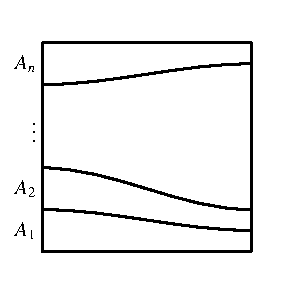
\includegraphics[width=0.3\hsize]{images/erwartung-4}
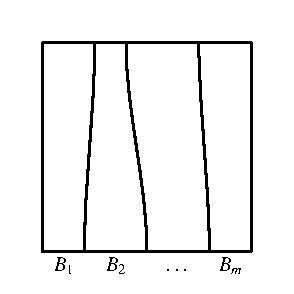
\includegraphics[width=0.3\hsize]{images/erwartung-3}
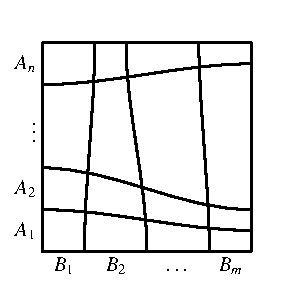
\includegraphics[width=0.3\hsize]{images/erwartung-2}
\end{center}
\caption{Ereignisse $A_i$ zur Berechung von $E(X)$, $B_j$ zur Berechnung
von $E(Y)$ und $A_i\cap B_j$ zur Berechnung von $E(XY)$.
\label{productexpectation}}
\end{figure}
Seien $A_i$ und $B_j$ Ereignisse so, dass $X$ auf den $A_i$ und $Y$ auf
den $B_j$ konstant ist. Dann kann man die Ereignisse $A_i\cap B_j$
zur Berechnung des Erwartungswertes heranziehen, wie in
Abbildung~\ref{productexpectation}, denn auf ihnen ist sowohl $X$ wie
auch $Y$ konstant.
Die Wahrscheinlichkeit von $A_i\cap B_j$ kann aber nur dann
durch die Wahrscheinlichkeiten von $A_i$ und $B_j$ ausgedr"uckt werden,
wenn die Ereignisse $A_i$ und $B_j$ paarweise
unabh"angig sind. Dann berechnet man:
\marginpar{\tiny\raggedright Rechenregel f"ur den Erwartungswert eines Produktes}
\begin{eqnarray*}
E(XY)&=&\sum_{i=1}^n\sum_{j=1}^m X(A_i\cap B_j)Y(A_i\cap B_j)P(A_i\cap B_j)\\
&=&\sum_{i=1}^n\sum_{j=1}^m X(A_i)Y(B_j)P(A_i)P(B_j)\\
&=&\sum_{i=1}^n X(A_i)P(A_i)\sum_{j=1}^mY(B_j)P(A_i)P(B_j)\\
&=&E(X)\cdot E(Y)
\end{eqnarray*}
Die oben verwendete Unabh"angigkeitsbedingung kann man mit folgender
Definition erzwingen:
\begin{definition}Zwei Zufallsvariable $X$ und $Y$ heissen
unabh"angig, wenn die Ereignisse $\{\omega|X(\omega)\le x\}$
und $\{\omega|Y(\omega)\le y\}$ f"ur alle $x,y\in\mathbb R$
unabh"angig sind, also
\[
P((X\le x)\wedge(Y\le y))=P(X\le x)\,P(Y\le y)\quad\forall x,y\in\mathbb{R}.
\]
\end{definition}
\index{Produktregel!f\"ur den Erwartungswert}
Damit haben wir auch f"ur Zufallsvariable eine Produktregel:
\begin{satz}
\label{produktregel-erwartungswert}
Sind $X$ und $Y$ unabh"angige Zufallsvariablen, dann gilt
\[
E(XY)=E(X)\cdot E(Y).
\]
F"ur zwei beliebige Funktionen $f$ und $g$ von $\mathbb{R}$ nach $\mathbb{R}$,
so dass $f(X)$ und $g(Y)$ immer noch Zufallsvariable sind, gilt
\[
E(f(X)g(Y))=E(f(X))E(g(Y)).
\]
\end{satz}
Seien $X$ und $Y$ die Augenzahlen beim W"urfeln mit zwei W"urfeln.
\marginpar{\tiny\raggedright Erwartungswert des Produktes der Augenzahlen
beim W"urfeln}
Die Ereignisse $X\le x$ und $Y\le y$ sind offensichtlich unabh"angig
(``horizontale und vertikale Streifen''), daher gilt
\[
E(XY)=E(X)E(Y)=3.5^2=12.25.
\]

\subsection{Erwartungswert und Integration}
\index{Erwartungswert!und Integration}
Die Berechnung des Erwartungswertes war im vorangegangene Abschnitt
einfach m"oglich, weil wir annehmen konnten, dass es Ereignisse $A$
gibt, auf denen die Zufallsvariable $X$ konstant ist. Wenn diese
Bedingung nicht mehr gilt, k"onnte man versuchen, den Erwartungswert
durch die Summe der kleinsten und gr"ossten m"oglichen Werte auf jedem
Ereignis $A_i$ einzuschachteln:
\[
\sum_{i=0}^nP(A_i)\min_{\omega\in A_i}X(\omega)
\le E(X)\le
\sum_{i=0}^nP(A_i)\max_{\omega\in A_i}X(\omega).
\]
Wir betrachten als Spezialfall die Ereignisalgebra f"ur eine
Messung, hier ist $\Omega=\mathbb{R}$. Die Wahrscheinlichkeitsfunktion $P$
liefert zu jedem Teilintervall $I\subset \mathbb{R}$ eine Wahrscheinlichkeit.
Wir betrachten eine Zerlegung der reellen Achse in Teilintervalle $I_i$.
Zu einer Funktion $X\colon \mathbb{R}\to\mathbb{R}$ kann man jetzt den
Erwartungswert wie folgt berechnen:
\[
\sum_{i=0}^nP(I_i)\min_{x\in I_i}X(x)
\le E(X)\le
\sum_{i=0}^nP(I_i)\max_{x\in I_i}X(x).
\]
Diese Konstruktion ist aber aus der Analysis vertraut, auf diese
Art wurde das Integral konstruiert. Die Summenausdr"ucke sind sogenannte
Riemannsche Summen, der einzige Unterschied ist, dass nicht die L"ange des
Intervalls, sondern die Wahrscheinlichkeit $P(I_i)$ des Intervalls gemessen
wird. Der Erwartungswert ist also eine Art verallgemeinertes Integral,
wof"ur der Mathematiker auch 
\[
E(X)=\int_{\Omega}X(\omega)dP(\omega)
\]
schreibt. Da uns diese Betrachtungsweise keine wirklich praktikablen
M"oglichkeiten zur Berechnung von $E(X)$ bietet, verfolgen wir sie
hier nicht weiter, werden aber im n"achsten Kapitel eine verwandte
Technik kennen lernen, welche nur gew"ohnliche Integrale verwendet.

\section{Varianz\label{section-varianz}}
\index{Varianz}
Die Qualit"atskontrolle bei der Herstellung von Widerst"anden versucht
ein Mass daf"ur zu entwickeln, wie genau die produzierten Widerst"ande
den beabsichtigen Widerstandswert einhalten. 
Dazu werden der Produktion einige Widerst"ande entnommen und ihr Wert
nachgemessen. Den Erwartungswert des Widerstandswertes kann man mit
Hilfe des Mittelwertes absch"atzen, er sollte ungef"ahr mit dem Sollwert
"ubereinstimmen.
\marginpar{\tiny\raggedright Varianz als Mass f"ur Streuung}
Wie aber kann man die ``Streuung'' der Widerstandswerte
bewerten?

Als weiteres Beispiel betrachten wir die die Zufallsvariable $X$
``Messung einer Spannung''. Nicht jede Messung ergibt den gleichen Wert,
\marginpar{\tiny\raggedright Varianz als Mass f"ur Rauschen}
das Signal ist von einem Rauschen "uberlagert. Der Mittelwert der
Messwert entspricht gem"ass dem vorangegangenen Abschnitt dem Erwartungswert
$E(X)$. Wie aber soll das Ausmass des Rauschens gemessen werden?
Ein praktischer Ansatz besteht darin, nach der Energie zu fragen, die
in dem Rauschsignal steckt. Die Leistung einer Wechselspannung $U(t)$
an einem Widerstand $R$ ist ja
$\frac{U(t)^2}R$, d.h. die mittlere Leistung w"ahrend des Intervalls $[t_0,t_1]$ 
ist
\[
\frac1{t_1-t_0}\int_{t_0}^{t_1}\frac{U(t)^2}R\,dt.
\]
Stellen wir uns vor, dass die Spannungsmessung $X$ in regelm"assigen, kurzen
Zeitintervallen wiederholt wird, dann ist die mittlere Leistung
des Differenzsignal $X-E(X)$ also proportional Summe der Quadrate
der Werte $(X-E(X))^2$, oder
\[
E((X-E(X))^2).
\]

\subsection{Definition}
\index{Varianz!Definition}
Die Einf"uhrungsbespiele motivieren folgende Definition:
\begin{definition}
\marginpar{\tiny\raggedright Definition der Varianz}
Sei $X\colon\Omega\to\mathbb{R}$ eine Zufallsvariable, dann
heisst die durch $\operatorname{var}(X)^2=E((X-E(X))^2)$ definierte Gr"osse $\operatorname{var}(X)$ die
{\bf Varianz} von $X$. Es ist insbesondere
\[
\operatorname{var}(X)=E((X-E(X))^2)=E(X^2)-E(X)^2
\]
\end{definition}
Die letzte Gleichung kann man leicht nachrechnen:
\begin{eqnarray*}
\operatorname{var}(X)&=&E((X-E(X))^2)\\
&=&E(X^2-2XE(X)+E(X)^2)\\
&=&E(X^2)-2E(X)E(X)+E(X)^2\\
&=&E(X^2)-E(X)^2\\
\end{eqnarray*}

\begin{figure}
\begin{center}
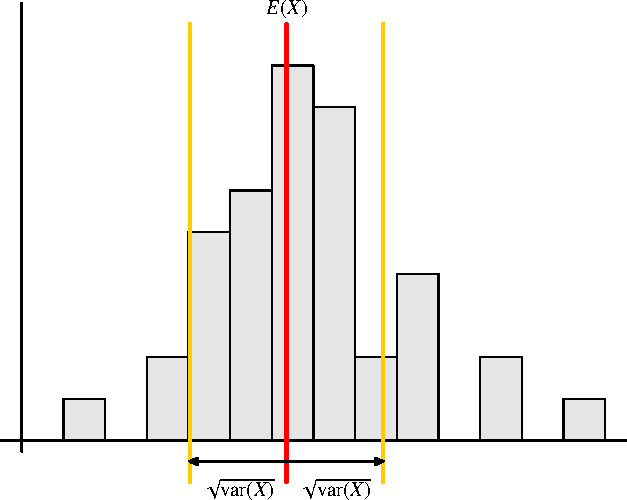
\includegraphics[width=\hsize]{images/erwartung-1}
\end{center}
\caption{Visualisierung von Erwartungswert und Varianz ein einem Histogramm
\label{histogram}}
\end{figure}

Man beachte, dass $\operatorname{var}(X)$ die Masseinheit des Quadrates
von $X$ hat.
Wenn also $X$ als Masseinheit eine L"ange hat,
dann hat $\operatorname{var}(X)$ die Masseinheit einer Fl"ache.
Insbesondere kann man $\operatorname{var}(X)$ nicht in der gleichen
Zeichnung visualisieren wie $E(X)$.
Aber die Gr"sse $\sqrt{\operatorname{var}(X)}$ hat die gleiche Masseinheit, sie
dr"uckt die ``Streubreite'' der Werte von $X$ aus,
wie in Abbildung~\ref{histogram} veranschaulicht.

Die Definition der Varianz ``passt'' in nat"urlicher Weise zum Erwartungswert,
wie der folgende Satz zeigt:
\begin{satz}\label{erwartungswert-charakterisierung}
\marginpar{\tiny\raggedright Minimumeigenschaft des Erwartungswertes}
Der Erwartungswert $E(X)$ einer reellen Zufallsvariable $X$ ist diejenige
reelle Zahl $\mu$, f"ur die $E((X-\mu)^2)$ minimal wird.
\end{satz}
\begin{proof}[Beweis]
Aus den Rechenregeln finden wir
\begin{eqnarray*}
E((X-\mu)^2)&=&E(X^2-2\mu X+\mu^2)\\
&=&E(X^2)-2\mu E(X) +\mu^2E(1)\\
&=&E(X^2)-2\mu E(X) +\mu^2P(\Omega)\\
&=&E(X^2)-2\mu E(X) +\mu^2
\end{eqnarray*}
Dies ist eine quadratische Funktion, die ihren Scheitelpunkt bei $\mu$ hat.
Man kann dies auch durch Nullsetzen der Ableitung nach $\mu$ finden:
\[
\frac{d}{d\mu}\left(E(X^2)-2\mu E(X) +\mu^2\right)=-2 E(X)+2\mu=0,
\]
Aufl"osen nach $\mu$ ergibt $\mu=E(X)$.
\end{proof}
Wir wenden die Definition der Varianz auf das Beispiel der Widerstandsmessung
an,
Wir haben bereits im Abschnitt \ref{erwartungswertvonmesswerten}
den Erwartungswert $E(R)=0.99015$ der Widerstandsmesswerte ermittelt, darauf aufbauend
k"onnen wir jetzt auch die Varianz berechnen.
Man findet zum Beispiel die Widerstandswerte gem"ass
Tabelle~\ref{varianzberechnung}.
\begin{table}
\begin{center}
\begin{tabular}{|c|r|r|r|}
\hline
Nummer&Messwert&Abweichung&$\text{Abweichung}^2$\\
\hline
1&0.990&-0.00015&0.0000000225\\
2&0.989&-0.00115&0.0000013225\\
3&0.991&0.00085&0.0000007225\\
4&0.991&0.00085&0.0000007225\\
5&0.991&0.00085&0.0000007225\\
6&0.989&-0.00115&0.0000013225\\
7&0.990&0.00015&0.0000000225\\
8&0.989&-0.00115&0.0000013225\\
9&0.992&0.00185&0.0000034225\\
10&0.992&0.00185&0.0000034225\\
11&0.990&-0.00015&0.0000000225\\
12&0.989&-0.00115&0.0000013225\\
13&0.990&-0.00015&0.0000000225\\
14&0.991&0.00085&0.0000007225\\
15&0.989&-0.00115&0.0000013225\\
16&0.990&-0.00015&0.0000000225\\
17&0.989&-0.00115&0.0000013225\\
18&0.990&-0.00015&0.0000000225\\
19&0.990&-0.00015&0.0000000225\\
20&0.991&0.00085&0.0000007225\\
\hline
&$\mu=1.000$&$\sigma=0.000963$&
$\sigma^2=0.0000009275$\\
\hline
\end{tabular}
\end{center}
\caption{Einzelmessungen an Widerst"anden und Berechnung der Varianz
\label{varianzberechnung}}
\end{table}

\subsubsection{Beispiel: Wurf einer fairen M"unze}
Beim Wurf einer fairen M"unze werde der Gewinn $1$ ausbezahlt bei
``Kopf'', bei ``Zahl'' wird hingegen $0$ ausbezahlt. Es ist klar,
dass die erwartete Auszahlung $E(X)=\frac12$ ist.
Daraus l"asst sich jetzt auch die Varianz berechnen:
\begin{align*}
\operatorname{var}(X)
&=
E((X-E(X))^2)=E\biggl(\biggl(X-\frac12\biggr)^2\biggr)
=\frac12\cdot \biggl(1-\frac12\biggr)^2+\frac12\biggl(0-\frac12\biggr)^2\\
&=\frac12\cdot\frac14+\frac12\cdot\frac14=\frac14.
\end{align*}

\subsection{Empirische Berechnung}
\index{Varianz!angen\"aherte Berechnung}
Wir betrachten das praktische Beispiel der Bestimmung der Varianz
\marginpar{\tiny\raggedright Berechnung der Varianz}
einer Messreihe.
Gegeben sind also die Messwerte $(x_i)_{1\le i\le n}$
Auf den ersten Blick sieht es so aus, als w"are f"ur die Berechnung der Varianz
sehr viel Speicherplatz erforderlich. Zwar ist f"ur die Berechnung des
Erwartungswertes von $\mu=E(X)=\frac1n\sum_{i=1}^n x_i$ kein besonderer Aufwand
notwendig, da die Summe laufend gebildet werden kann. Zur Berechnung der
Varianz muss aber erst $\mu$ bestimmt werden, bevor man die Differenzen $(x_i-\mu)$
bilden kann. Trotzdem l"asst sich die Berechnung vereinfachen:
\begin{eqnarray*}
E((X-\mu)^2)&=&\frac1n\sum_{i=1}^n(x_i-\mu)^2\\
&=&\frac1n\sum_{i=1}^n(x_i^2-2\mu x_i+\mu^2)\\
&=&\frac1n\sum_{i=1}^nx_i^2-2\mu\frac1n\sum_{i=1}^n x_i+\mu^2\\
&=&\frac1n\sum_{i=1}^nx_i^2-\bigl(\frac1n\sum_{i=1}^nx_i\bigr)^2\\
\end{eqnarray*}
\subsubsection{Beobachtungen}
\begin{enumerate}
\item
Es gen"ugt also, $x_i$ und $x_i^2$ zu summieren, wozu nur zwei Speicherpl"atze
ben"otigt werden.
Aus den beiden Summen kann die Varianz bereits berechnet werden.
Es ist nicht n"otig, die einzelnen Messwerte $x_i$ zu speichern.
\item
Die Berechnung der Varianz kann also ganz einfach mit einer Tabelle
erfolgen:
\begin{center}
%\begin{tabular}{|>{$}c<{$}|>{$}c<{$}|}
\begin{tabular}{|c|c|c|}
\hline
$i$&$x_i$&$x_i^2$\\
\hline
$1$&$x_1$&$x_1^2$\\
$2$&$x_2$&$x_2^2$\\
$\vdots$&$\vdots$&$\vdots$\\
$n$&$x_n$&$x_n^2$\\
\hline
&$\sum_{i=0}^n x_i$&$\sum_{i=0}^n x_i^2$\\
\hline
\end{tabular}
\end{center}
\item
Grosse Abweichungen k"onnen vorkommen, und bekommen wegen des
Quadrates in der Varianz auch grosses Gewicht. Hat man aber nur
wenige Messwerte, ist es unwahrscheinlich, eine solche grosse
Abweichung, einen ``Ausreisser'', zu sehen. Daher untersch"atzt
diese empirische Formel den tats"achlichen Wert der Varianz immer
dann, wenn $n$ klein ist. Wir werden sp"ater sehen, dass eine
besser Sch"atzung zu bekommen ist, wenn man noch einen Korrekturfaktor
$\frac{n}{n-1}$ hinzuf"ugt.
\end{enumerate}

\subsection{Weitere Rechenregeln}
\begin{satz}
\label{rechenregeln-varianz}
Seien $X$ und $Y$ unabh"angige Zufallsvariable, dann haben
Summe und Produkt folgende Varianz:
\begin{eqnarray*}
\operatorname{var}(\lambda X)&=&\lambda^2\operatorname{var}(X)\\
\operatorname{var}(X+Y)&=&\operatorname{var}(X)+\operatorname{var}(Y)\\
\operatorname{var}(XY)&=&\operatorname{var}(X)\operatorname{var}(Y)
+
\operatorname{var}(Y)E(X)^2+\operatorname{var}(X)E(Y)^2
\end{eqnarray*}
\end{satz}
\begin{proof}[Beweis]Durch einfaches Nachrechnen unter Ausn"utzen der
Rechenregeln f"ur den Erwartungswert und der
Unabh"angigkeit von $X$ und $Y$, d.h. $E(XY)=E(X)E(Y)$:
\begin{eqnarray*}
\operatorname{var}(X+Y)
&=&E((X+Y)^2)-E(X+Y)^2\\
&=&E(X^2+2XY+Y^2)-(E(X)+E(Y))^2\\
&=&E(X^2)+2E(XY)+E(Y^2)-E(X)^2-2E(X)E(Y)-E(Y)^2\\
&=&E(X^2)-E(X)^2+E(Y^2)-E(Y)^2\\
&=&\operatorname{var}(X)+\operatorname{var}(Y)
\end{eqnarray*}
Durch ziehen der Wurzel folgt die Behauptung aus der letzten Gleichung.
F"ur das Produkt gilt
\begin{eqnarray*}
\operatorname{var}(XY)
&=&E(X^2Y^2)-E(XY)^2\\
&=&E(X^2)E(Y^2)-E(X)^2E(Y)^2\\
&=&(\operatorname{var}(X)+E(X)^2))(\operatorname{var}(Y)+E(Y)^2)
-E(X)^2E(Y)^2\\
&=&\operatorname{var}(X)\operatorname{var}(Y)+E(X)^2\operatorname{var}(Y)
+\operatorname{var}(X)E(Y)^2
\end{eqnarray*}
und daraus die Behauptung.
\end{proof}

\subsubsection{Beobachtungen}

\begin{enumerate}
\item
Die Varianz funktioniert "ahnlich wie das Quadrieren f"ur gew"ohnliche Zahlen.
Schreibt man $E(XY)-E(X)E(Y)=\operatorname{cov}(X,Y)$, lautete die
binomische Formel wird f"ur die Varianz:
\begin{equation}
\operatorname{var}(X+Y)=\operatorname{var}(X)
+2\operatorname{cov}(X,Y)
+\operatorname{var}(Y).
\label{var-summe-abhaengig}
\end{equation}
Die Kovarianz $\operatorname{cov}(X,Y)$ spielt also die Rolle des gemischten
Terms in der ``ge"ohnliche'' binomischen Formel.
\item
Sind $X$ und $Y$ unabh"angig, gilt daher die Formel
\begin{align*}
\operatorname{var}(X+Y)
&=
\operatorname{var}(X)
+
\operatorname{var}(Y)
\\
\sqrt{\operatorname{var}(X+Y)}
&=
\sqrt{
\sqrt{\operatorname{var}(X)}^2
+
\sqrt{\operatorname{var}(Y)}^2
}
\end{align*}
Die Gr"ossen $\sqrt{\operatorname{var}(X)}$ und $\sqrt{\operatorname{var}(Y)}$
werden daher wie die Katheten eines rechtwinkligen Dreiecks addiert,
man spricht von {\it pythator"aischer} Addition.
\end{enumerate}

\subsubsection{Anwendung: Wurf von $n$ M"unzen}
Sei $X$ die Anzahl ``Kopf'' beim Wurf von $n$ M"unzen. Nat"urlich wird
$X$ nur Werte zwischen $0$ und $n$ annehmen.
Zur Berechnung von $E(X)$ und $\operatorname{var}(X)$ wollen wir
die Rechenregeln verwenden. Dabei verwenden wir neue Zufallsvariablen
$X_i$ wie folgt:
\begin{center}
\begin{tabular}{clcc}
$X_1$&Anzahl Kopf im ersten Wurf&$E(X_1)=\frac12$&$\operatorname{var}(X_1)=\frac14$\\
$X_2$&Anzahl Kopf im zweiten Wurf&$E(X_2)=\frac12$&$\operatorname{var}(X_2)=\frac14$\\
&$\dots$&&\\
$X_n$&Anzahl Kopf im $n$-ten Wurf&$E(X_n)=\frac12$&$\operatorname{var}(X_n)=\frac14$\\
\end{tabular}
\end{center}
Damit kann man Erwartungswert und Varianz von $X=X_1+X_2+\dots+X_n$ berechnen:
\begin{align*}
E(X)&=
E(X_1)+
E(X_2)+\dots+
E(X_n)
=
\frac{1}2+
\frac{1}2+\dots+
\frac{1}2=\frac{n}2
\\
\operatorname{var}(X)
&=
\operatorname{var}(X_1)
+
\operatorname{var}(X_2)
+\dots+
\operatorname{var}(X_n)
=\frac14+\frac14+\dots+\frac14=\frac{n}4.
\end{align*}

\section{Wie genau ist der Mittelwert?}
Der Erwartungswert dr"uckt aus, wie gross eine Zufallvariable ``im Mittel''
sein wird.
Je gr"osser aber die Varianz ist, desto gr"osser wird die Abweichung
der Zufallsvariable vom ``mittleren Wert'' sein.
Wie misst man diese Abweichung? Mit der Varianz haben wir bereits
ein Mass f"ur die mittlere Abweichung, aber noch keinen Hinweis
darauf, wie h"aufig grosse Abweichungen vorkommen werden.

Sei $\mu=E(X)$ der Erwartungswert der Zufallsvariablen $X$.
F"ur die Varianz hatten wir die Abweichung $X-\mu$ der Zufallsvariablen
von ihrem Erwartungswert untersucht.
Meistens wird die Abweichung klein sein. Uns interessiert jetzt aber,
wie wahrscheinlich es ist, dass sie gross ist.
Sei $\varepsilon>0$ ein Schwellwert f"ur die Abweichung, wir m"ochten
also wissen, wie h"aufig die Abweichung $\varepsilon$ "uberschreitete:
\[
|X-\mu|>\varepsilon.
\]
Wir m"ochten die Wahrscheinlichkeit 
\[
P(|X-\mu|>\varepsilon)
\]
berechnen.
Nach unseren einleitenden Bemerkungen sollte es einen Zusammenhang
zwischen Varianz und und dieser Wahrscheinlichkeit geben: je gr"osser
die Varianz, desto gr"osser die Wahrscheinlichkeit einer grossen
Abweichung.

\subsection{Ungleichung von Tschebyscheff}\label{ungleichung-von-tschebyscheff}
\index{Tschebyscheff!Ungleichung von}
Selbst wenn man gar nichts "uber die Zufallsvariable weiss, ausser
dass sie eine Varianz besitzt, kann man eine Aussage "uber die 
Wahrscheinlichkeit einer grossen Abweichung machen.
Dies ist der Inhalt der Ungleichung von Tschebyscheff.
Dies kann nat"urlich
nur eine grobe obere Schranke sein, f"ur genaue Resultate muss man
mehr "uber das konkrete Experiment wissen.
\marginpar{\tiny\raggedright Wahrscheinlichkeit f"ur Abweichung vom Erwartungswert}

\begin{satz}[Ungleichung von Tschebyscheff]
Ist eine Zufallsvariable $X$, dann l"asst sich die Wahrscheinlichkeit,
dass $X$ um mehr als $\varepsilon$ vom Erwartungswert abweicht, wie
folgt absch"atzen:
\[
P(|X-\mu| >\varepsilon)\le\frac{\operatorname{var}(X)}{\varepsilon^2}
\]
\end{satz}

L"asst man $\varepsilon$ wachsen findet man, dass Abweichungen
deutlich gr"osser als $\sqrt{\operatorname{var}(X)}$ 
sehr unwahrscheinlich sind.

\begin{proof}[Beweis]
Sei $A =\{\omega\;|\;|X(\omega)-\mu|>\varepsilon\}$ das Ereignis, dass die
Zufallsvariable $X$ um mehr als $\varepsilon$ vom Mittelwert abgewichen
ist. Offensichtlich ist dies dasselbe, wie wenn $(X-\mu)^2$ mehr als
$\varepsilon^2$ von 0 abweicht. Es gilt daher:
\[
\varepsilon^2 \chi_{A} \le (X-\mu)^2
\]
Wenden wir darauf den Erwartungswert an, folgt
\[
\varepsilon^2 P(A)\le E((X-\mu)^2)=\operatorname{var}(X)
\]
Die Tschebyscheffsche Ungleichung folgt jetzt nach Division durch
$\varepsilon^2$.
\end{proof}
Beispiel:
\marginpar{\tiny\raggedright Anwendung: Produktions"uberwachung}
Bei der Herstellung von 1k$\Omega$ Widerst"anden
m"ochte man sicherstellen,
dass nur bei 1\% aller produzierten Widerst"ande der Wert um mehr als
10$\Omega$ vom Sollwert abweicht. Um das zu "uberpr"ufen entnimmt man der
Produktion eine Stichprobe, und sch"atzt die Varianz ab. Wie gross darf die
Varianz maximal werden, damit die Bedingung noch erf"ullt ist?

Die Tschebyscheffsche Ungleichung liefert in diesem Fall
\[
\operatorname{var}(X)\ge\varepsilon^2P(|X-\mu| >\varepsilon)
\]
oder
\[
\operatorname{var}(X)\ge 10^2\cdot 0.01=1.
\]
Sobald die Varianz der Stichprobe gr"osser als 1$\Omega^2$ ist, kann die
Tschebyscheffungleichung die Einhaltung der Qualit"atsvorgabe nicht
mehr garantieren.

Die Tschebyscheff-Ungleichung ist bei weitem nicht die bestm"ogliche.
\marginpar{\tiny\raggedright Grenzen der Tschebyscheff-Ungleichung}
Fragt man zum Beispiel nach der Wahrscheinlichkeit, dass $X$ um mehr
als zwei Standardabweichungen, also um mehr als $2\sqrt{\operatorname{var}(X)}$ vom
Erwartungswert abweicht, dann liefert sie
\[
P(|X-\mu|>2\sqrt{\operatorname{var}(X)})
\le\frac{\operatorname{var}(X)}{2^2\operatorname{var}(X)}=\frac14.
\]
Diese Ungleichung gilt f"ur jede Zufallsvariable $X$.
Es gibt aber Zufallsvariablen, f"ur die 
\[
P(|X-\mu|>2\sqrt{\operatorname{var}(X)})\le 0.05,
\]
Wir werden mit der Normalverteilung solche Zufallsvariablen kennenlernen.
Auf das Beispiel angewendet bedeutet dies, dass die Tschebyscheff-Ungleichung
m"oglicherweise viel zu oft behauptet, dass die Produktionsqualit"at ungen"ugend
ist, weil die Widerstandswerte vermutlich in guter N"aherung normalverteilt
sein werden.

\subsection{Wie gut approximiert der Mittelwert den Erwartungswert?}
\label{approximation-mittelwert}
Wir betrachten eine Folge von unabh"angigen Zufallsvariablen $X_1, X_2,\dots$, die
alle den gleichen Erwartungswert $E(X_i)=\mu$ und die gleiche Varianz
$\operatorname{var}(X_i)=\sigma^2$ haben. Dann erwartet man, dass 
der Mittelwert der ersten $n$ Zufallsvariablen, also die
\marginpar{\tiny\raggedright Mittelwert von Zufallsvariablen}
Gr"osse
\[
M_n=\frac{X_1+X_2+\dots+X_n}{n}
\]
eine gut N"aherung ist f"ur $\mu$. Trotzdem kann es vorkommen, wegen
einzelner Ausreisser unter den $X_i$ der Mittelwert recht weit weg
vom Mittelwert liegt. Der folgende Satz von Bernoulli sagt, wie wahrscheinlich
es ist, dass der Mittelwert weiter als $\varepsilon$ vom Erwartungswert
entfernt ist.

Zun"achst halten wir fest, dass
\[
M_n=\frac{X_1+\dots+X_n}{n}
\]
eine Zufallsvariable ist mit Erwartungswert
\[
E(M_n)=E\biggl(\frac{X_1+\dots+X_n}{n}\biggr)
=\frac{E(X_1)+\dots+E(X_n)}{n}=\mu
\]
und Varianz
\[
\operatorname{var}(M_n) =\frac1{n^2}\sum_{i=1}^n\operatorname{var}(X_i)
=\frac{\sigma^2}n,
\]
wie man mit den Rechenregeln f"ur die Varianz sofort nachrechnet.

\index{Gesetz der grossen Zahlen}
\index{Bernoulli!Gesetz der grossen Zahlen}
\begin{satz}[Bernoullis Gesetz der grossen Zahlen]
Die Wahrscheinlichkeit, dass der Mittelwert von $n$ unabh"angigen Zufallsvariablen
mit Erwartungswert $\mu$ und Varianz $\sigma^2$ mehr als $\varepsilon$ von $\mu$
abweicht ist
\[
P(|M_n-\mu|>\varepsilon)\le \frac{\sigma^2}{\varepsilon^2n}.
\]
Insbesondere gilt
\[
\lim_{n\to\infty}P(|M_n-\mu|>\varepsilon)=0.
\]
\end{satz}
\begin{proof}[Beweis]
Aus der Tschebyscheffschen Ungleichung folgt:
\[
P(|M_n-\mu|>\varepsilon)\le\frac{\operatorname{var}(M_n)}{\varepsilon^2}=
\frac{\sigma^2}{n\varepsilon^2}.
\]
Dies entspricht genau der Behauptung.
\end{proof}
Leider sind die Vorhersagen wie auch bei der Tschebyscheff-Ungleichung
nur beschr"ankt n"utzlich. Wenn die Wahrscheinlichkeit, dass der Mittelwert
um mehr als $\sigma$ vom Erwartungswert abweicht, kleiner als 1\% sein
soll, sind daf"ur nach dem Gesetz der grossen Zahlen mindestens 100 Summanden
n"otig.

\subsection{Wie genau ist die empirische H"aufigkeit?}
Wir haben durch Wiederholung von Experimenten auch versucht, die
Wahrscheinlichkeit eines Ereignisses durch die H"aufigkeit zu approximieren,
mit welcher dieses Ereignis eintritt.
Mit dem Satz von Bernoulli ist es uns jetzt auch m"oglich, die
Wahrscheinlichkeit daf"ur abzusch"atzen, dass wir ein falsches
Resultat erhalten.
\begin{satz}
Wird ein Experiment $n$ mal durchgef"uhrt, und tritt dabei das Ereignis $A$
mit der relativen H"aufigkeit $h$ ein, dann ist die Wahrscheinlichkeit,
dass $h$ um mehr als $\varepsilon$ von $P(A)$ abweicht
\[
P(|h- P(A)|>\varepsilon)\le \frac{P(A)(1-P(A))}{n\varepsilon^2}
\le\frac{1}{4n\varepsilon^2}
\]
\end{satz}
\begin{proof}[Beweis]
Wir betrachten die Zufallsvariablen $X_i$, welche den Wert $1$ hat,
wenn im $i$-ten Versuch das Ereignis $A$ eingetreten ist, und sonst $0$.
Diese Zufallsvariablen sind offensichtlich unabh"angig. Betrachtet man
nur die einzelne Durchf"uhrung $i$ des Versuches, dann ist $X_i$
die Funktion
$\chi_A$, welchen
den Erwartungswert $E(\chi_A)=P(A)$, und die Varianz ist
\begin{eqnarray*}
\operatorname{var}(\chi_A)&=&E(\chi_A^2)-E(\chi_A)^2=E(\chi_A)-E(\chi_A)^2\\
&=&P(A)-P(A)^2=P(A)(1-P(A))
\end{eqnarray*}
hat.
Der Mittelwert $M_n$ ist die Anzahl der Versuche, bei denen das Ereignis
$A$ eingetreten ist, geteilt durch $n$, also die Anzahl aller Versuche,
$h=M_n$. Damit folgt aus dem Gesetz der grossen Zahlen:
\[
P(|h-P(A)|>\varepsilon)\le\frac{P(A)(1-P(A))}{n\varepsilon^2}.
\]
Die letzte Ungleichung des Satzes folgt aus der Tatsache, dass die Funktion
$p\mapsto p(1-p)=p-p^2$ bei $p=\frac12$ ein Maximum hat, also
$P(A)(1-P(A))\le\frac14$ gilt.
\end{proof}
Insbesondere verstehen wir jetzt, warum es sehr lange dauern kann, bis
wir durch Z"ahlen der H"aufigkeit eines Ereignisses dessen Wahrscheinlichkeit
auch nur auf wenige Stellen nach dem Komma bestimmen k"onnen. Wenn wir
verlangen, dass die relative H"aufigkeit mit
99\% Sicherheit die Wahrscheinlichkeit auf drei Stellen ann"ahert, also
$\varepsilon=10^{-3}$, dann m"ussen wir verlangen
\begin{eqnarray*}
\frac{1}{4n\varepsilon^2}&\le&0.01\\
\frac1{4\cdot 10^{-3\cdot 2}\cdot10^{-2}}=25\cdot 10^6&\le&n.
\end{eqnarray*}
Der Versuch muss also mindestens 25 Millionen mal wiederholt werden,
um eine Genauigkeit von drei Stellen nach dem Komma mit 99\% Sicherheit
zu erreichen. Dies deckt sich mit den Beobachtungen in der W"urfelsimulation
in Tabelle
\ref{wuerfel-simulation}.
\section{Lineare Regression}
\index{Regression!lineare}
\index{lineare Regression}
\index{Kurvenanpassung}
\begin{figure}
\begin{center}
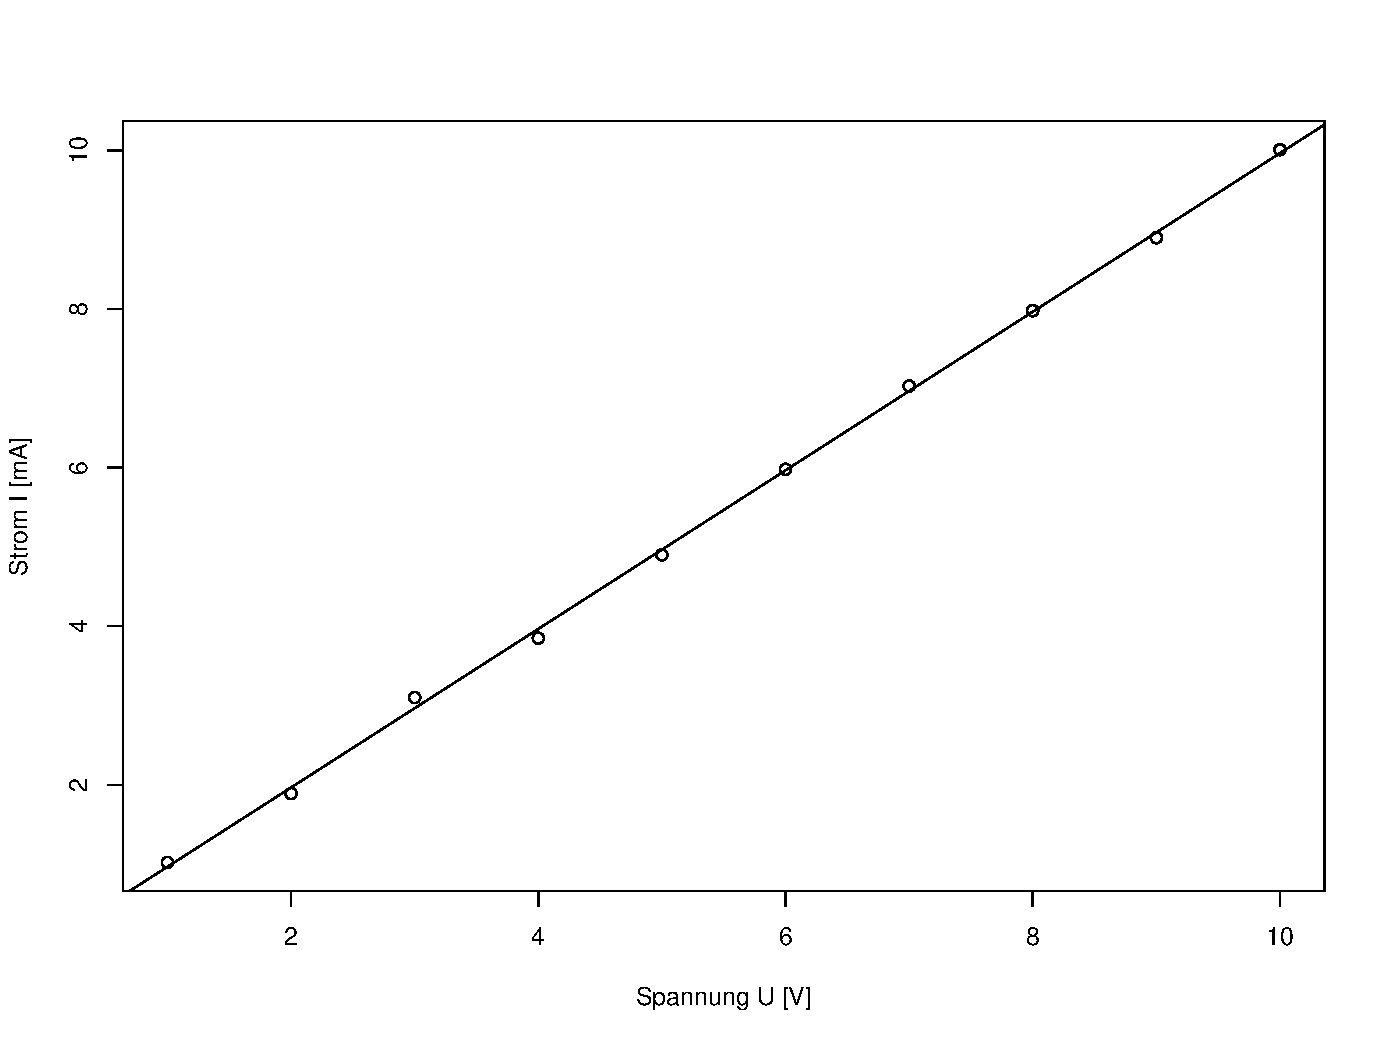
\includegraphics[width=0.8\hsize]{graphics/ohm}
\end{center}
\caption{Anpassung einer Geraden an gemessen Strom-/Spannungs-Werte\label{ohm-regression}}
\end{figure}
Der Satz \ref{erwartungswert-charakterisierung} hat gezeigt, dass der
Erwartungswert jener Wert ist, der die Varianz minimiert. Diese Idee
l"asst sich auch auf kompliziertere Zusammenh"ange anwenden. In einem
Stromkreis erwartet man auf Grund des Ohmschen Gesetzes, dass Spannung $U$
und Strom $I$ proportional sind: $U=RI$. F"uhrt man eine Messung von beiden
Gr"ossen durch, erh"alt man zwei Zufallsvariablen $U(\omega)$ und $I(\omega)$,
und die Proportionalit"at wird wegen der Messfehler meistens nicht mehr
erf"ullt sein. Wie gross ist der Widerstansdwert $R$? Es w"are zwar denkbar,
f"ur jede Messung den Widerstandswert zu errechnen, und dann das Mittel
zu bilden. Noch besser ist aber, den Widerstandswert $R$ so zu bestimmen,
dass der erwartete quadratische Fehler
$E( (U-RI)^2)$
m"oglichst klein ist.
\marginpar{\tiny\raggedright Regressionsgerade als lineare N"aherung f"ur einen Datensatz}
Abbildung \ref{ohm-regression} zeigt eine solche Gerade.


\subsection{Regressionsgerade}
Etwas allgemeiner finden wir folgenden Satz "uber die sogenannte
Regressionsgerade:
\begin{satz}
\label{rekursion}
Seien $X$ und $Y$ zwei reelle Zufallsvariable. Die Gerade mit der
Gleichung $y=ax+b$ minimiert die Varianz
$\operatorname{var}(aX+b-Y)$ genau dann, wenn 
\begin{eqnarray*}
a&=&\frac{E(XY)-E(X)E(Y)}{(E(X^2)-E(X)^2)}=\frac{\operatorname{cov}(X,Y)}{\operatorname{var}(X)}\\
b&=&E(Y)-E(X)a
\end{eqnarray*}
\end{satz}
\begin{proof}[Beweis]
Der mittlere quadratische Fehler ist
\begin{eqnarray*}
Q(a,b)&=&E((aX+b-Y)^2)\\
&=&E(a^2X^2+b^2+Y^2+2abX-2aXY -2bY)\\
&=&a^2E(X^2)+b^2+E(Y^2)+2abE(X)-2aE(XY)-2bE(Y)
\end{eqnarray*}
Um das Minimum zu finden, setzen wir die partiellen Ableitungen nach $a$
und $b$ gleich Null, und finden:
\begin{eqnarray*}
0=\frac{\partial Q}{\partial a}&=&2aE(X^2)+2bE(X)-2E(XY)\\
0=\frac{\partial Q}{\partial b}&=&2b+2aE(X)-2E(Y)\\
\end{eqnarray*}
Dies ist gleichbedeutend mit dem folgenden linearen Gleichungssystem f"ur
die Koeffizienten
$a$ und $b$
\begin{alignat*}{4}
E(X^2)a\,&+\,&E(X)b\,&=\,&E(XY)\\
E(X)a\,&+&b\,&=&E(Y)
\end{alignat*}
Multipliziert man die zweite Gleichung mit $E(X)$ und subtrahiert sie von der
ersten, erh"alt man eine Gleichung f"ur $a$:
\begin{eqnarray*}
(E(X^2)-E(X)^2)a&=&E(XY)-E(X)E(Y)\\
a&=&\frac{E(XY)-E(X)E(Y)}{(E(X^2)-E(X)^2)} 
\end{eqnarray*}
Aus der zweiten Gleichung kann man nun auch $b$ finden:
\[
b=E(Y)-E(X)a
\]
womit alles bewiesen ist.
\end{proof}
Die Gleichung f"ur $b$ hat eine unmittelbare Konsequenz: die Regressionsgerade
geht immer durch den Punkt $(E(X), E(Y))$. In der Tat, damit der Punkt
$(E(X), E(Y))$ auf der Geraden liegt, muss die Bedinung $E(Y)=aE(X)+b$
erf"ullt sein. Schafft man $aE(X)$ auf die linke Seite, wird daraus
$E(Y)-aE(X)=b$, also genau die Gleichung f"ur $b$.

\subsubsection{Der mittlere quadratische Fehler}
Der mittlere quadratische Fehler l"asst sich nat"urlich auch berechnen.
Wir sind von $\operatorname{var}(Y-aX-b)$ als zu optimierender
Gr"osse ausgegangen. Inzwischen haben wir $a$ und $b$ bestimmt,
also k"onnen wir auch den Fehler berechnen. Dazu sind die Rechenregeln
hilfreich:
\begin{align*}
\operatorname{var}(Y-aX-b)
&=
\operatorname{var}(Y) + 
\operatorname{var}(-aX) + 
\operatorname{var}(-b)
+2\operatorname{cov}(-aX,Y)
\\
&=
\operatorname{var}(Y)+a^2\operatorname{var}(X)-2a\operatorname{cov}(X,Y)
\\
&=
\operatorname{var}(Y)
+ \frac{\operatorname{cov}(X,Y)^2}{\operatorname{var}(X)^2}\operatorname{var}(X)
-2 \frac{\operatorname{cov}(X,Y)}{\operatorname{var}(X)}\operatorname{cov}(X,Y)
\\
&=
\operatorname{var}(Y)-\frac{\operatorname{cov}(X,Y)^2}{\operatorname{var}(X)}
\end{align*}
Im zweiten Schritt mussten wir die Formel (\ref{var-summe-abhaengig})
verwenden, da die Zufallsvariablen $X$ und $Y$ nicht unabh"angig sind.

Nat"urlich
ist der Fehler 
wahrscheinlich ungef"ahr proportional zur Varianz der $Y$-Werte,
ohne Varianz gibt's auch keinen Fehler. Wir versuchen daher den Term
$\operatorname{var}(Y)$ auszuklammern:
\begin{align*}
\operatorname{var}(Y-aX-b)
&=
\operatorname{var}(Y)\left(1-\frac{\operatorname{cov}(X,Y)^2}{\operatorname{var}(X)\operatorname{var}(Y)}\right).
\end{align*}
Der Bruch wird damit ein nat"urliches Qualit"atsmass f"ur die Regressionsgerade:
\begin{definition}
\marginpar{\tiny\raggedright Definition des Regressionskoeffizienten}
Der Quotient
\[
r=\frac{\operatorname{cov}(X,Y)}{\sqrt{\operatorname{var}(X)\operatorname{var}(Y)}}
\]
heisst Regressionskoeffizient.
\end{definition}

Die Regression ist also umso genauer, je n"aher $r$ bei $\pm 1$ liegt.
Ausserdem hat $r$ immer das gleiche Vorzeichen wie die
Steigung der Regressionsgeraden.

\subsubsection{Berechnung aus empirischen Daten}
Auch die Koeffizienten der Regressionsgeraden sind mit einfachen Formeln
\marginpar{\tiny\raggedright Regressions-Formeln f"ur endliche Messreihen}
zu bestimmen, wenn man nur Messwerte, deren Quadrate und das Produkt summiert:
\begin{eqnarray*}
a&=&\frac{\displaystyle n\sum_{i=1}^nx_iy_i-\sum_{i=1}^nx_i\sum_{i=1}^ny_i}{\displaystyle n\sum_{i=1}^nx_i^2-\biggl(\sum_{i=1}^nx_i\biggr)^2}\\
b&=&\frac1n\sum_{i=1}^ny_i-a\frac1n\sum_{i=1}^nx_i\\
\end{eqnarray*}

\subsection{Anwendungsbeispiel}
\begin{table}
\begin{center}
\begin{tabular}{|c|c|}
\hline
Zeit [s]&L"ange [mm]\\
\hline
6&10.98\\
10&13.89\\
14&16.23\\
18&18.57\\
\hline
\end{tabular}
\end{center}
\caption{L"ange der Verz"ogerungselemente f"ur K1100T in Abh"angigkeit von der
Verz"ogerungszeit\label{delaylengths}}
\end{table}
Modellraketenmotoren auf Feststoffbasis verwenden ein Verz"ogerungselement,
welches nach Abbrand das eigentlichen Treibsstoffs noch einige Sekunden
weiter brennt, um dann eine Schwarzpulverladung zu z"unden, die einen Fallschirm
auswerfen kann. Die Verz"ogerungselemente werden nur f"ur wenige, diskrete
Verz"ogerungszeiten hergestellt. Ist kein passendes Verz"ogerungselement
verf"ugbar, muss
ein l"angeres Verz"ogerungselement durch Verk"urzung auf die passende
Verz"ogerungszeit eingestellt werden. Dazu muss jedoch der Zusammenhang
zwischen Verz"ogerungszeit und l"ange des Elementes bekannt sein.
Der Hersteller macht die Angaben in Tabelle \ref{delaylengths}.

\subsubsection{Berechnung von Hand}
Die Berechnung auf dem Papier kann man zum Beispiel mit Hilfe
\marginpar{\tiny\raggedright Berechnungsschema f"ur Regression von Hand}
des Berechnungsschemas gem"ass folgender Tabelle
organisieren, welche auch alle relevanten Formeln zeigt:
\begin{center}
\begin{tabular}{|l|l|l|l|}
\hline
$E(T)$&&&\\
$E(T^2)$&\footnotesize$\operatorname{var}(T)=E(T^2)-E(T)^2$&&\\
\hline
$E(L)$&&&\\
$E(L^2)$&\footnotesize$\operatorname{var}(L)=E(L^2)-E(L)^2$&&\\
\hline
$E(TL)$&\footnotesize$\operatorname{cov}(T,L)=E(TL)-E(T)E(L)$&$a=\frac{\operatorname{cov}(T,L)}{\operatorname{var}(T)}$&\footnotesize$b=E(L)-aE(T)$\\
&&$r=\frac{\operatorname{cov}(T,L)}{\sqrt{\operatorname{var}(T)\operatorname{var}(L)}}$&\\
\hline
\end{tabular}
\end{center}
Die Durchf"uhrung der Rechnung f"uhrt zu folgendem Resultat:
\begin{center}
\begin{tabular}{|r|r|r|r|}
\hline
12.0000&&&\\
164.0000&20.0000&&\\
\hline
14.9175&&&\\
230.4376&7.9058&&\\
\hline
191.5650&12.5550&0.627750&7.38450\\
&&0.998456&\\
\hline
\end{tabular}
\end{center}
Somit kann man als N"aherungsformel f"ur die L"ange des Verz"ogerungselements
die lineare Funktion
\[
l=0.62775 \cdot t+7.3845
\]
verwenden. Der mittlere quadratische Fehler dieser N"aherung ist
\[
\Delta = \operatorname{var}(L)(1-r^2)=0.024.
\]
Der L"angenfehler ist also etwa $\sigma_L=\sqrt{0.024}=0.15$mm, was einer
Ungenauigkeit der Verz"ogerungsdauer von 0.25s entspricht. Angesichts
der Fertigungs- und Betriebs\-toleranzen von bis zu 20\%, verursacht durch
Schwankungen in Abmessungen, physikalischen Eigenschaften des Treibstoffs
und Temperatur beim Abbrand ist dies bei weitem genau genug.
\subsubsection{Berechnung mit R}
\begin{figure}
\begin{center}
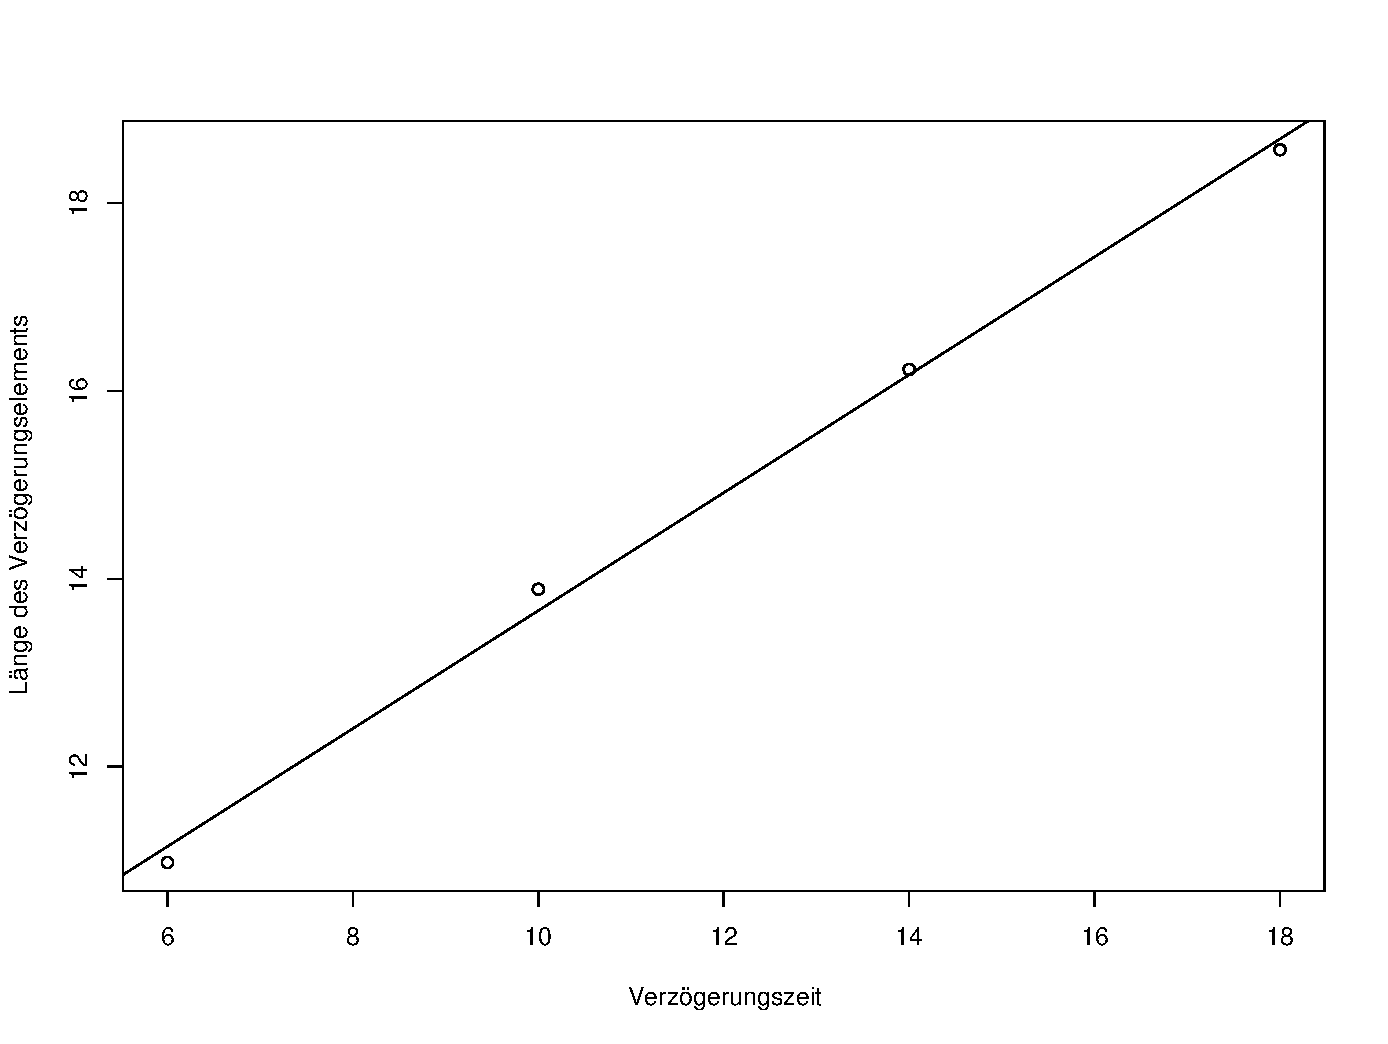
\includegraphics[width=0.7\hsize]{graphics/verzoegerungszeit}
\end{center}
\caption{Von R erzeugte graphische Darstellung der Regressionsgerade
f"ur die Verz"ogerungszeit\label{verzoegerungszeit}}
\end{figure}
Die Software R
\marginpar{\tiny\raggedright Statistik-Software R}
ist ein leistungsf"ahiges freies Softwarepaket f"ur statistische
Berechnungen. Mit folgenden Befehlen kann das obige Regressionsproblem
mit R gel"ost, und die Graphik
Graphik \ref{verzoegerungszeit} dargestellt
werden:

{\footnotesize
\begin{verbatim}
> zeit = c(6,10,14,18)
> laenge = c(10.98, 13.89, 16.23, 18.57)
> laenge.lm = lm(laenge ~ zeit)
> summary(laenge.lm)

Call:
lm(formula = laenge ~ zeit)

Residuals:
     1      2      3      4 
-0.171  0.228  0.057 -0.114 

Coefficients:
            Estimate Std. Error t value Pr(>|t|)   
(Intercept)  7.38450    0.31608   23.36  0.00183 **
zeit         0.62775    0.02468   25.43  0.00154 **
---
Signif. codes:  0 `***' 0.001 `**' 0.01 `*' 0.05 `�'0.1 ` ' 1 

Residual standard error: 0.2208 on 2 degrees of freedom
Multiple R-Squared: 0.9969,	Adjusted R-squared: 0.9954 
F-statistic: 646.9 on 1 and 2 DF,  p-value: 0.001542 

> plot(laenge ~ zeit, xlab="Verzoegerungszeit",
  ylab="Laenge des Verzoegerungselements")
> abline(laenge.lm)
\end{verbatim}}
}
R kann von \url{http://www.r-project.org} heruntergeladen werden.
